\section{Generative Models and Naive Bayes}

\subsection{Probability Fundamentals}

\begin{definition}{Probability Basics}
Key probability concepts include:
\begin{itemize}
    \item \textbf{Sample Space} ($S$): Set of all possible outcomes
    \item \textbf{Event}: Subset of the sample space
    \item \textbf{Probability of an Event} ($P(A)$): Measure of how likely event $A$ is to occur
    \item \textbf{Axioms}: Non-negativity, certainty ($P(S) = 1$), and additivity
\end{itemize}
\end{definition}

\begin{definition}{Joint and Conditional Probability}
\begin{itemize}
    \item \textbf{Joint Probability}: $P(A \cap B)$ is the probability of events $A$ and $B$ occurring together
    \item \textbf{Conditional Probability}: $P(B|A) = \frac{P(A \cap B)}{P(A)}$ is the probability of event $B$ given that event $A$ has occurred
    \item \textbf{Independence}: Events $A$ and $B$ are independent if $P(A \cap B) = P(A) \cdot P(B)$
\end{itemize}
\end{definition}

\mult{2}

\begin{definition}{Bayes' Theorem}\\
Bayes' theorem describes how to update probabilities based on new evidence:
\[P(A|B) = \frac{P(B|A) \cdot P(A)}{P(B)}\]
where:
\begin{itemize}
    \item $P(A|B)$ is the posterior probability
    \item $P(B|A)$ is the likelihood
    \item $P(A)$ is the prior probability
    \item $P(B)$ is the evidence
\end{itemize}
\end{definition}

\begin{concept}{Law of Total Probability}\\
The law of total probability relates the probability of an event to conditional probabilities:
\[P(A) = \sum_{i=1}^{n} P(A|B_i)P(B_i)\]
where $B_1, B_2, ..., B_n$ form a partition of the sample space (mutually exclusive and collectively exhaustive).
\end{concept}
\multend

\subsection{Parameter Estimation}

\mult{2}

\begin{definition}{Parameter Estimation}
\begin{itemize}
    \item \textbf{Maximum Likelihood Estimation (MLE)}: Finds parameter values that maximize the likelihood of observing the training data
    \item \textbf{Maximum A Posteriori (MAP)}: Incorporates prior beliefs about parameters, finding values that maximize the posterior probability
\end{itemize}
\end{definition}


\begin{definition}{Likelihood Function}
The likelihood function measures how well a statistical model (with given parameters) explains observed data:
\[L(\theta; X) = P(X|\theta)\]
For independent observations, it's the product of individual probabilities:
\[L(\theta; X) = \prod_{i=1}^{n} P(x^{(i)}|\theta)\]
\end{definition}

\begin{example}{MLE for Bernoulli Distribution}
Consider estimating the probability of heads for a biased coin:
\begin{itemize}
    \item Data: 7 heads and 3 tails in 10 flips
    \item Model: Bernoulli distribution with parameter $p$ (probability of heads)
    \item Likelihood: $L(p; X) = p^7 (1-p)^3$
    \item Log-likelihood: $\log L(p; X) = 7\log(p) + 3\log(1-p)$
    \item Derivative: $\frac{\partial}{\partial p} \log L(p; X) = \frac{7}{p} - \frac{3}{1-p}$
    \item Setting to zero: $\frac{7}{p} - \frac{3}{1-p} = 0$
    \item Solving: $p_{MLE} = \frac{7}{10} = 0.7$
\end{itemize}
\end{example}

\begin{KR}{Maximum Likelihood Estimation}
\paragraph{Define the likelihood function}
Express the probability of observing the data given the parameters:
\[L(\theta; X) = P(X|\theta) = \prod_{i=1}^{n} P(x^{(i)}|\theta)\]

\paragraph{Take the logarithm}
Convert to log-likelihood for easier computation:
\[\log L(\theta; X) = \sum_{i=1}^{n} \log P(x^{(i)}|\theta)\]

\paragraph{Find the maximum}
Set the derivative to zero and solve for parameters:
\[\frac{\partial}{\partial \theta} \log L(\theta; X) = 0\]

\paragraph{Check for maximum}
Verify second derivative is negative to ensure maximum
\end{KR}



\multend

\subsection{Generative vs. Discriminative Models}

\begin{definition}{Generative Models}\\
Generative models learn the joint probability distribution $P(X, Y)$ of inputs $X$ and labels $Y$. They model how the data is generated and can generate new samples:
\begin{itemize}
    \item Learn $P(X|Y)$ (likelihood) and $P(Y)$ (prior)
    \item Use Bayes' theorem to calculate $P(Y|X)$ for predictions
    \item Examples include Naive Bayes and Hidden Markov Models
\end{itemize}
\end{definition}

\begin{definition}{Discriminative Models}\\
Discriminative models directly learn the conditional probability $P(Y|X)$ or the mapping from inputs to outputs:
\begin{itemize}
    \item Focus on decision boundaries between classes
    \item Don't model the data generation process
    \item Examples include Logistic Regression, SVM, and Neural Networks
\end{itemize}
\end{definition}

\begin{concept}{Comparing Generative and Discriminative Models}
\begin{itemize}
    \item \textbf{Data efficiency}: Generative models often perform better with less data
    \item \textbf{Expressiveness}: Generative models capture the full distribution
    \item \textbf{Accuracy}: Discriminative models typically achieve better classification accuracy
    \item \textbf{Outlier detection}: Generative models can identify outliers as low-probability instances
    \item \textbf{Missing features}: Generative models can handle missing features naturally
\end{itemize}
\end{concept}

\begin{example2}{Generative vs. Discriminative Approach}
Consider a simple email classification task:
\begin{itemize}
    \item Task: Classify emails as spam or not spam
    \item Features: Presence of words like ''money'', ''free'', ''meeting''
\end{itemize}
\tcblower
Discriminative approach (Logistic Regression):
\begin{itemize}
    \item Directly models: $P(\text{spam}|\text{words})$
    \item Learns weights for each word that predict spam probability
    \item Example function: $P(\text{spam}|\text{words}) = \sigma(0.8 \times \text{money} + 0.9 \times \text{free} - 0.7 \times \text{meeting})$
\end{itemize}

Generative approach (Naive Bayes):
\begin{itemize}
    \item Models: $P(\text{words}|\text{spam})$ and $P(\text{spam})$
    \item Learns how likely each word appears in spam and non-spam
    \item For example: $P(\text{money}|\text{spam}) = 0.3$, $P(\text{money}|\text{not spam}) = 0.05$
    \item Uses Bayes' theorem: $P(\text{spam}|\text{words}) = \frac{P(\text{words}|\text{spam})P(\text{spam})}{P(\text{words})}$
\end{itemize}
\end{example2}

\raggedcolumns
\columnbreak

\subsection{Naive Bayes Classifier}

\mult{2}

\begin{definition}{Naive Bayes}\\
Naive Bayes is a probabilistic classifier based on Bayes' theorem with a ''naive'' independence assumption between features:
\[P(Y|X) = \frac{P(X|Y) \cdot P(Y)}{P(X)}\]
The naive assumption allows us to write:
\[P(X|Y) = \prod_{i=1}^{n} P(X_i|Y)\]
This simplifies calculations significantly.
\end{definition}

\begin{theorem}{Advantages and Disadvantages of Naive Bayes}\\
Advantages:
\begin{itemize}
    \item Simple and fast to train
    \item Works well with high-dimensional data
    \item Performs well with small training sets
    \item Handles missing values naturally
\end{itemize}
Disadvantages:
\begin{itemize}
    \item Independence assumption is often violated in real data
    \item Not suitable for regression problems
    \item May be outperformed by more sophisticated models for complex tasks
    \item Probability estimates may be unreliable
\end{itemize}
\end{theorem}

\multend

\begin{concept}{Types of Naive Bayes}\\
Different implementations of Naive Bayes exist for different types of data:
\begin{itemize}
    \item \textbf{Bernoulli Naive Bayes}: For binary features (presence/absence)
    \item \textbf{Multinomial Naive Bayes}: For discrete features (e.g., word counts)
    \item \textbf{Gaussian Naive Bayes}: For continuous features, assuming normal distribution
\end{itemize}
\end{concept}

\begin{KR}{Implementing Naive Bayes}
\paragraph{Calculate prior probabilities}
Compute $P(Y=y_k)$ for each class $y_k$ based on their frequency in the training data

\paragraph{Calculate likelihoods}
For each feature $X_i$ and class $y_k$, compute the likelihood $P(X_i|Y=y_k)$:
\begin{itemize}
    \item For discrete features (Multinomial NB): Use frequency counts
    \item For binary features (Bernoulli NB): Use presence/absence frequencies
    \item For continuous features (Gaussian NB): Estimate using Gaussian distribution
\end{itemize}

\paragraph{Apply Bayes' theorem for prediction}
For a new instance $x$, calculate for each class $y_k$:
\[P(Y=y_k|X=x) \propto P(Y=y_k) \prod_{i=1}^{n} P(X_i=x_i|Y=y_k)\]
Predict the class with highest posterior probability.
\end{KR}



\begin{concept}{Laplace Smoothing}\\
Laplace smoothing (or additive smoothing) addresses the zero-probability problem:
\begin{itemize}
    \item Problem: If a feature value never appears in a class during training, its likelihood is zero
    \item Solution: Add a small count (typically 1) to all feature values
    \item Formula: $P(X_i=x_i|Y=y_k) = \frac{count(X_i=x_i, Y=y_k) + \alpha}{count(Y=y_k) + \alpha \cdot |V|}$
    \item Where $|V|$ is the number of possible values for feature $X_i$ and $\alpha$ is the smoothing parameter
\end{itemize}
\end{concept}


\begin{KR}{Text Classification with Naive Bayes}
\paragraph{Preprocess text}
\begin{itemize}
    \item Tokenize text into words
    \item Remove stop words (optional)
    \item Apply stemming or lemmatization (optional)
    \item Create feature vectors (e.g., bag of words, TF-IDF)
\end{itemize}

\paragraph{Train Multinomial Naive Bayes}
\begin{itemize}
    \item Calculate class priors $P(C_k)$
    \item Calculate word likelihoods $P(w_i|C_k)$ for each word and class
    \item Apply Laplace smoothing to handle unseen words
\end{itemize}

\paragraph{Classify new documents}
\begin{itemize}
    \item Tokenize and preprocess
    \item Apply Bayes' theorem using log probabilities to avoid underflow
    \item Assign document to class with highest probability
\end{itemize}
\end{KR}


\begin{example2}{Naive Bayes Text Classification}
    $$
    \begin{gathered}
    C_1=\text { buys }_{\text {computer }}=\text { yes }, \quad C_2=\text { buys }_{\text {computer }}=\text { no } \\
    X=\left(\text { age }=\text { youth } ; \text { income }=\text { med } ; \text { student }=\text { yes } ; \text { credit }_{\text {rating }}=\text { fair }\right)
    \end{gathered}
    $$

    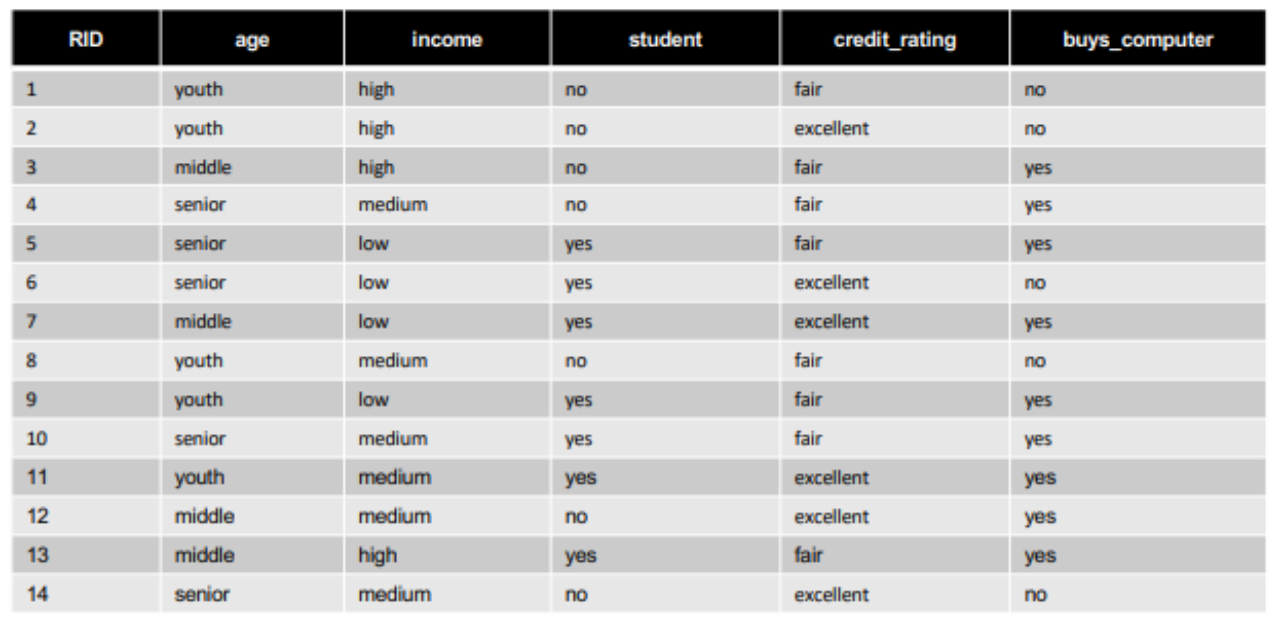
\includegraphics[width=\linewidth]{naive_bayes_example.png}

    \textbf{Compute $P\left(C_i\right)$}

$$
P\left(C_1\right)=0.643, \quad P\left(C_2\right)=0.357
$$


\textbf{Compute $P\left(X \mid C_i\right)$}
\begin{itemize}
    \item $P\left(X \mid C_1\right)=P\left(\right.$ age $=$ youth $\left.\mid C_1\right) \cdot P\left(\right.$ income $=$ med $\left.\mid C_1\right) \ldots=0.044$
    \item $P\left(X \mid C_1\right)=P\left(\right.$ age $=$ youth $\left.\mid C_1\right) \cdot P\left(\right.$ income $=$ med $\left.\mid C_1\right) \ldots=0.044$
\end{itemize}

\textbf{Compute $P\left(X \mid C_i\right) \cdot P\left(C_i\right)$}
\begin{itemize}
    \item $P\left(X \mid C_1\right) \cdot P\left(C_1\right)=0.044 \cdot 0.643=0.028$
    \item $P\left(X \mid C_2\right) \cdot P\left(C_2\right)=0.019 \cdot 0.357=0.007$
\end{itemize}
    
\end{example2}

